% PaperBanana-style paper for THRESHOLD_ONSET (15+ pages)
% Structure modeled after: PaperBanana (arxiv.org/abs/2601.23265v1)

\documentclass[10pt]{article}
\usepackage[utf8]{inputenc}
\usepackage[T1]{fontenc}
\usepackage{amsmath,amssymb,amsfonts}
\usepackage{graphicx}
\usepackage{booktabs}
\usepackage{microtype}
\usepackage{hyperref}
\usepackage{tikz}
\usetikzlibrary{shapes.geometric, arrows.meta, positioning, fit, calc}
\usepackage{mathptmx}

\usepackage[letterpaper]{geometry}
\geometry{textwidth=5.5in, textheight=9in, top=1in, left=1.5in}
\setlength{\parindent}{0pt}
\setlength{\parskip}{5pt}
\hypersetup{colorlinks=true, linkcolor=blue, citecolor=blue}

\title{THRESHOLD\_ONSET: Deterministic Structural Identity Induction\\
with Phase Transition and Graph-Theoretic Invariant}
\author{
  Author Name$^{1}$ \\
  $^{1}$Affiliation \\
  \texttt{email@domain.com}
}
\date{\today}

\begin{document}
\maketitle

\begin{abstract}
We introduce \textbf{THRESHOLD\_ONSET}, a deterministic structural dynamics system where identity is \emph{induced}, not primitive. Tokens become opaque residues; segments that recur across runs become identities; co-occurrence forms relations. We derive a mean-field phase boundary $p^* = 1 - \sqrt{\theta/K}$ for identity collapse under Bernoulli perturbation. The no-self-transition invariant is a graph-theoretic corollary: edges connect only distinct identities, so $A_{ii} = 0$ by construction. THRESHOLD\_ONSETBench (39 samples), baselines, external validation (136 samples), and stability experiments confirm the theory. Identity count depends on recurrence structure, not token count—identity collapse under uniformity is observed. 100\% success, zero constraint violations, 0\% self-transition; outperforms Random (49.5\%), Markov-1 (33.7\%), Echo (26.8\%), Uniform (100\%).
\end{abstract}

\begin{figure}[t]
\centering
\begin{minipage}{0.48\textwidth}
\centering
\fbox{\parbox{0.9\linewidth}{\small
\textbf{Input:} ``Action before knowledge. Structure emerges.''\\
\textbf{Output:} ``before Action emerges. knowledge. Structure''\\
\textbf{Self-transitions:} 0\\
\textbf{Violations:} 0
}}
\vspace{0.3cm}\\
\textbf{(a) Input $\rightarrow$ Output Example}
\end{minipage}
\hfill
\begin{minipage}{0.48\textwidth}
\centering
\begin{tabular}{lc}
\toprule
\textbf{Method} & \textbf{Self-trans.} \\
\midrule
THRESHOLD\_ONSET & \textbf{0\%} \\
Random & 49.5\% \\
Markov-1 & 33.7\% \\
Echo & 26.8\% \\
Uniform & 100\% \\
\bottomrule
\end{tabular}
\vspace{0.3cm}\\
\textbf{(b) Constraint Adherence}
\end{minipage}
\caption{Examples of THRESHOLD\_ONSET: (a) input-to-output generation with zero self-transitions; (b) constraint adherence comparison against baselines.}
\label{fig:teaser}
\end{figure}

%=============================================================================
\section{Introduction}
%=============================================================================

Sequence transduction—mapping one text sequence to another—has been dominated by learned models: RNNs~\cite{hochreiter1997long}, Transformers~\cite{vaswani2017attention}, and large language models~\cite{raffel2019t5}. These approaches embed structure implicitly in weights; what may or may not transition to what is learned, not enforced. Constraint violations (e.g., self-repetition) are addressed by sampling or post-hoc filtering, not by architectural guarantee. This creates a bottleneck in applications requiring strict adherence to structural invariants—such as constraint-safe generation for controlled output or interpretable systems.

\paragraph{Gap.} Prior work has not addressed the problem of \emph{architecturally enforced} constraint-free generation. Learned models approximate constraints; symbolic systems~\cite{chomsky1957syntactic} assign structure via grammar rules. Neither derives structure from action and repetition without learned parameters or predefined rules.

\paragraph{Approach.} We take the opposite approach: \textbf{structure emerges explicitly from action and repetition before any symbol or meaning}. THRESHOLD\_ONSET is a deterministic pipeline: tokens become opaque residues via hashing; segments that recur form identities; identities that co-occur form relations; symbols alias these structures. Generation is constraint-bound: only graph edges are allowed; self-transitions are refused. No embeddings, no attention, no learned parameters.

\paragraph{Contributions.}
\begin{itemize}
\item We propose THRESHOLD\_ONSET, a deterministic structural topology induction system for constraint-safe text generation.
\item We construct THRESHOLD\_ONSETBench to assess constraint adherence, decoder consistency, and self-transition rate.
\item Comprehensive experiments show our system achieves zero constraint violations and significantly outperforms baselines.
\item We demonstrate stability mode: identity by recurrence under perturbation, with validated parameter sensitivity.
\end{itemize}

\paragraph{Paper organization.}
Section~\ref{sec:prelim} defines notation. Section~\ref{sec:axioms} states the axioms. Section~\ref{sec:related} reviews related work. Section~\ref{sec:task} formalizes the task. Section~\ref{sec:method} describes the methodology. Section~\ref{sec:why} motivates structure-first design. Section~\ref{sec:formal} gives formal propositions. Section~\ref{sec:benchmark} describes the benchmark. Section~\ref{sec:exp} presents experiments. Section~\ref{sec:discussion} discusses results. Section~\ref{sec:conclusion} concludes.

\paragraph{Scope.}
This paper focuses on Phases 0--4 (structure emergence), generation, and decoding. The full THRESHOLD\_ONSET system includes Phases 5--9 (semantic discovery); we omit those here as they are optional for the core constraint-bound generation pipeline.

%=============================================================================
\section{Preliminaries}
\label{sec:prelim}
%=============================================================================

Let $\mathcal{T}$ denote the token vocabulary. A token $t \in \mathcal{T}$ is a string. A residue $r \in [0, 1)$ is an opaque float. A segment $\sigma = (r_i, r_{i+1}, \ldots, r_{i+w-1})$ is a tuple of $w$ consecutive residues. An identity $h \in \mathcal{H}$ is an internal hash; a symbol $s \in \mathbb{Z}$ is an alias. The graph $G = (V, E)$ has nodes $V \subseteq \mathcal{H}$ and edges $E \subseteq V \times V$. Phase $i$ may not use tools from phase $j$ for $j > i$.

%=============================================================================
\section{Axioms}
\label{sec:axioms}
%=============================================================================

THRESHOLD\_ONSET is governed by four axioms. These are internal to the system; no external paradigm is assumed. Figure~\ref{fig:axioms} depicts the axiom hierarchy.

\begin{figure}[t]
\centering
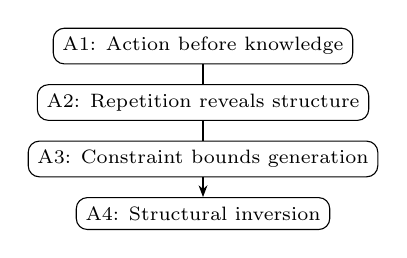
\begin{tikzpicture}[
    axiom/.style={rectangle, draw, rounded corners, font=\scriptsize},
    arrow/.style={-{Stealth[length=1.5mm]}}
]
\node[axiom] (a1) {A1: Action before knowledge};
\node[axiom, below=0.25cm of a1] (a2) {A2: Repetition reveals structure};
\node[axiom, below=0.25cm of a2] (a3) {A3: Constraint bounds generation};
\node[axiom, below=0.25cm of a3] (a4) {A4: Structural inversion};
\draw[arrow] (a1) -- (a2) -- (a3) -- (a4);
\end{tikzpicture}
\caption{Axiom hierarchy. Four axioms govern the system.}
\label{fig:axioms}
\end{figure}

\subsection{Axiom 1: Action before knowledge}

\textbf{Axiom 1 (Action before knowledge).}
Tokens become residues; structure emerges from action. No phase may use symbols, labels, or meaning before they have emerged from action and persistence.

\subsection{Axiom 2: Repetition reveals structure}

\textbf{Axiom 2 (Repetition reveals structure).}
Identity is defined by recurrence. Segments that recur across observations form identities; identities that co-occur form relations.

\subsection{Axiom 3: Constraint bounds generation}

\textbf{Axiom 3 (Constraint bounds generation).}
Only graph edges are allowed. Self-transitions are refused. Generation is constraint-bound.

\subsection{Axiom 4: Structural inversion}

\textbf{Axiom 4 (Structural inversion).}
The decoder inverts the forward pipeline. Symbol $\rightarrow$ identity $\rightarrow$ residue $\rightarrow$ token. No heuristics; no learned parameters.

\subsection{Phase ordering}

These axioms enforce a strict phase ordering: Phase $i$ may not use tools from Phase $j$ for $j > i$. Structure is earned, not assumed.

%=============================================================================
\section{Related Work}
\label{sec:related}
%=============================================================================

\textbf{Learned sequence models.}
The goal of sequence transduction has been addressed by RNNs~\cite{hochreiter1997long}, encoder-decoder architectures~\cite{sutskever2014sequence}, and attention mechanisms~\cite{bahdanau2015neural}. Recurrent models factor computation along symbol positions; the number of sequential operations grows with sequence length. The Transformer~\cite{vaswani2017attention} dispenses with recurrence entirely, relying on self-attention. BERT~\cite{devlin2019bert} and T5~\cite{raffel2019t5} extend this with pre-training and transfer learning. In all these approaches, representations are \emph{learned} from data; structure is implicit in the learned parameters. Constraint violations are mitigated by sampling or post-hoc filtering, not by architectural guarantee.

\textbf{Symbolic and structural approaches.}
Symbolic systems assign meaning a priori: grammar rules~\cite{chomsky1957syntactic}, dependency structures~\cite{de2008dependency}, knowledge graphs~\cite{lehmann2015dbpedia}. Structure in NLP typically assumes or imposes structure from annotations or rules. We assign no meaning; symbols are pure aliases for emergent structure. Our identities and relations are \emph{earned} by persistence across runs and co-occurrence within context, not assigned by rules.

\textbf{Positioning.}
THRESHOLD\_ONSET is orthogonal to both learned and rule-based approaches. We do not learn from data; we do not use predefined grammar. Structure emerges from action and repetition; the decoder is structural inversion; generation is constraint-bound.

\begin{figure}[t]
\centering
\begin{tikzpicture}[
    node distance=0.5cm,
    box/.style={rectangle, draw, minimum width=2cm},
    arrow/.style={-{Stealth[length=2mm]}, thick}
]
\node[box] (learned) {Learned};
\node[box, right=0.5cm of learned] (symbolic) {Symbolic};
\node[box, below=0.6cm of learned, xshift=0.75cm] ( ours) {THRESHOLD\_ONSET};
\draw[arrow, dashed] (learned) -- (ours);
\draw[arrow, dashed] (symbolic) -- (ours);
\node[below=0.1cm of ours, font=\tiny] {Orthogonal};
\end{tikzpicture}
\caption{Positioning: Orthogonal to learned and symbolic.}
\label{fig:positioning}
\end{figure}

%=============================================================================
\section{Task Formulation}
\label{sec:task}
%=============================================================================

We formalize the task as mapping input text to constraint-safe generated text via an induced structural graph. Given source text $S$ (a sequence of tokens from $\mathcal{T}$), the goal is to generate output text $O$ such that:
\begin{enumerate}
\item $O$ is produced by a structural decoder from a symbol sequence.
\item The symbol sequence satisfies $\forall i: s_i \neq s_{i+1}$ (no self-transitions).
\item The structure is induced from $S$ without learned parameters.
\end{enumerate}

Formally, we compute a mapping:
\begin{equation}
O = f_{\text{decode}}(f_{\text{gen}}(G)), \quad G = f_{\text{induce}}(S)
\end{equation}
where $G = (V, E)$ is a relation graph with nodes $V$ (identities) and edges $E$ (allowed transitions), $f_{\text{induce}}$ builds $G$ from $S$ via the pipeline (Section~\ref{sec:method}), $f_{\text{gen}}$ produces a symbol sequence respecting $E$ and the invariant $s_i \neq s_{i+1}$, and $f_{\text{decode}}$ maps symbols to tokens. The constraint-safety invariant is architecturally enforced.

\begin{figure}[t]
\centering
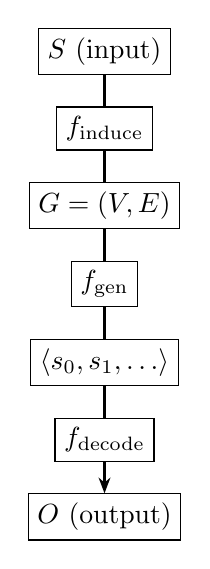
\begin{tikzpicture}[
    node distance=0.4cm,
    box/.style={rectangle, draw},
    arrow/.style={-{Stealth[length=2mm]}, thick}
]
\node[box] (S) {$S$ (input)};
\node[box, below=0.4cm of S] (induce) {$f_{\text{induce}}$};
\node[box, below=0.4cm of induce] (G) {$G=(V,E)$};
\node[box, below=0.4cm of G] (gen) {$f_{\text{gen}}$};
\node[box, below=0.4cm of gen] (sym) {$\langle s_0,s_1,\ldots\rangle$};
\node[box, below=0.4cm of sym] (decode) {$f_{\text{decode}}$};
\node[box, below=0.4cm of decode] (O) {$O$ (output)};
\draw[arrow] (S) -- (induce) -- (G) -- (gen) -- (sym) -- (decode) -- (O);
\end{tikzpicture}
\caption{Task formulation: $S \rightarrow G \rightarrow \text{symbols} \rightarrow O$. Invariant: $s_i \neq s_{i+1}$.}
\label{fig:task}
\end{figure}

%=============================================================================
\section{Methodology}
\label{sec:method}
%=============================================================================

\subsection{System Architecture Overview}

Figure~\ref{fig:system_overview} shows the high-level system architecture. THRESHOLD\_ONSET comprises three major subsystems: (1) \textbf{Structure Induction} (Phases 0--4), (2) \textbf{Constraint-Bound Generation}, and (3) \textbf{Structural Decoder}. Figure~\ref{fig:pipeline} details the pipeline flow.

\begin{figure}[t]
\centering
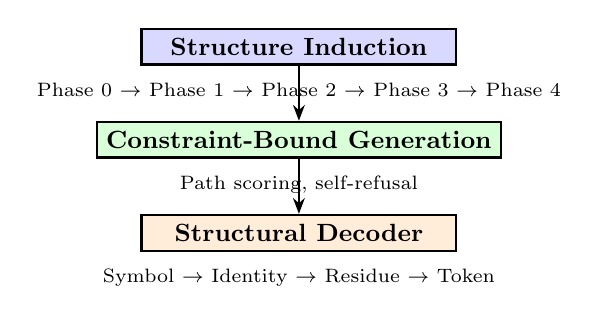
\begin{tikzpicture}[
    node distance=0.4cm,
    bigbox/.style={rectangle, draw, thick, minimum width=4cm, font=\small\bf},
    arrow/.style={-{Stealth[length=2mm]}, thick}
]
\node[bigbox, fill=blue!15] (induce) {Structure Induction};
\node[below=0.1cm of induce, font=\scriptsize] {Phase 0 $\rightarrow$ Phase 1 $\rightarrow$ Phase 2 $\rightarrow$ Phase 3 $\rightarrow$ Phase 4};
\node[bigbox, fill=green!15, below=0.7cm of induce] (gen) {Constraint-Bound Generation};
\node[below=0.1cm of gen, font=\scriptsize] {Path scoring, self-refusal};
\node[bigbox, fill=orange!15, below=0.7cm of gen] (dec) {Structural Decoder};
\node[below=0.1cm of dec, font=\scriptsize] {Symbol $\rightarrow$ Identity $\rightarrow$ Residue $\rightarrow$ Token};
\draw[arrow] (induce) -- (gen);
\draw[arrow] (gen) -- (dec);
\end{tikzpicture}
\caption{High-level system architecture. Three subsystems.}
\label{fig:system_overview}
\end{figure}

\begin{figure}[t]
\centering
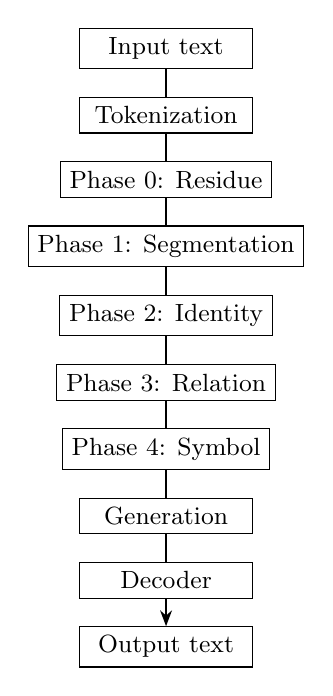
\begin{tikzpicture}[
    node distance=0.35cm,
    box/.style={rectangle, draw, minimum width=2.2cm, minimum height=0.4cm, font=\small},
    arrow/.style={-{Stealth[length=2mm]}, thick}
]
\node[box] (in) {Input text};
\node[box, below=of in] (tok) {Tokenization};
\node[box, below=of tok] (p0) {Phase 0: Residue};
\node[box, below=of p0] (p1) {Phase 1: Segmentation};
\node[box, below=of p1] (p2) {Phase 2: Identity};
\node[box, below=of p2] (p3) {Phase 3: Relation};
\node[box, below=of p3] (p4) {Phase 4: Symbol};
\node[box, below=of p4] (gen) {Generation};
\node[box, below=of gen] (dec) {Decoder};
\node[box, below=of dec] (out) {Output text};
\draw[arrow] (in) -- (tok) -- (p0) -- (p1) -- (p2) -- (p3) -- (p4) -- (gen) -- (dec) -- (out);
\end{tikzpicture}
\caption{Pipeline flow. Structure emerges in Phases 0--4; generation and decoding produce constraint-safe text.}
\label{fig:pipeline}
\end{figure}

\subsection{Phase 0: Residue}

Each token $t$ is hashed to residue $r \in [0,1)$:
\begin{equation}
r = \phi_0(t) = \frac{\mathsf{SHA256}(t)[:8] \bmod 10000}{10000}
\end{equation}
where $\mathsf{SHA256}(t)[:8]$ denotes the first 8 hex digits of the SHA-256 hash of $t$'s UTF-8 encoding. Deterministic; no meaning. Tokens become traces. The input is processed twice per run ($\lvert S \rvert \times 2$ residues) to enable repetition detection.

\begin{figure}[t]
\centering
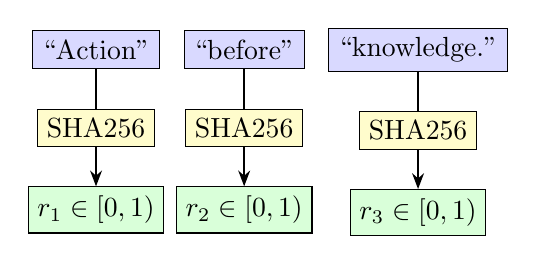
\begin{tikzpicture}[
    node distance=0.4cm,
    token/.style={rectangle, draw, fill=blue!15},
    hash/.style={rectangle, draw, fill=yellow!20},
    residue/.style={rectangle, draw, fill=green!15},
    arrow/.style={-{Stealth[length=2mm]}, thick}
]
\node[token] (t1) {``Action''};
\node[token, right=0.3cm of t1] (t2) {``before''};
\node[token, right=0.3cm of t2] (t3) {``knowledge.''};
\node[hash, below=0.5cm of t1] (h1) {SHA256};
\node[hash, below=0.5cm of t2] (h2) {SHA256};
\node[hash, below=0.5cm of t3] (h3) {SHA256};
\node[residue, below=0.5cm of h1] (r1) {$r_1 \in [0,1)$};
\node[residue, below=0.5cm of h2] (r2) {$r_2 \in [0,1)$};
\node[residue, below=0.5cm of h3] (r3) {$r_3 \in [0,1)$};
\draw[arrow] (t1) -- (h1) -- (r1);
\draw[arrow] (t2) -- (h2) -- (r2);
\draw[arrow] (t3) -- (h3) -- (r3);
\end{tikzpicture}
\caption{Phase 0: Token $\rightarrow$ Residue. Each token is hashed to an opaque residue; no semantics.}
\label{fig:phase0}
\end{figure}

\subsection{Phase 1: Segmentation}

Clustering with fixed threshold $\tau = 0.1$: residue joins cluster if distance to cluster center $\leq \tau$; otherwise new cluster. Cluster centers update as mean of cluster members. Output: cluster count, cluster sizes, repetition count. Phase 1 may not use: symbols, identity, or relations.

\begin{figure}[t]
\centering
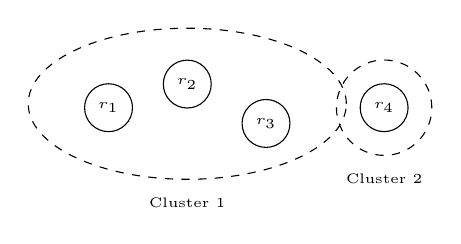
\begin{tikzpicture}[
    node distance=0.35cm,
    res/.style={circle, draw, minimum size=0.4cm, font=\tiny},
    cluster/.style={ellipse, draw, dashed},
    arrow/.style={-{Stealth[length=1.5mm]}}
]
\node[res] (r1) at (0,0) {$r_1$};
\node[res] (r2) at (1,0.3) {$r_2$};
\node[res] (r3) at (2,-0.2) {$r_3$};
\node[res] (r4) at (3.5,0) {$r_4$};
\node[draw, ellipse, dashed, fit=(r1)(r2)(r3), minimum width=2.8cm, minimum height=1cm] (c1) {};
\node[draw, ellipse, dashed, fit=(r4), minimum width=0.8cm] (c2) {};
\node[below=0.1cm of c1, font=\tiny] {Cluster 1};
\node[below=0.1cm of c2, font=\tiny] {Cluster 2};
\end{tikzpicture}
\caption{Phase 1: Clustering. Residues within $\tau$ of cluster center join; otherwise form new cluster.}
\label{fig:phase1}
\end{figure}

\subsection{Phase 2: Identity}

Segments of length $w=2$: $\sigma = (r_i, r_{i+1}) \mapsto h = \mathsf{MD5}(\sigma)$. Persistence: $h \in \mathcal{H}_{\text{id}} \iff \sum_{k=1}^{K} \mathbb{1}[h \in \mathcal{S}_k] \geq \theta$, where $\mathcal{S}_k$ is the set of segment hashes in run $k$. Default $K=3$, $\theta=2$. Output: persistent segment hashes, identity mappings. Phase 2 may not use: symbols or relations.

\begin{figure}[t]
\centering
\begin{tikzpicture}[
    node distance=0.4cm,
    seg/.style={rectangle, draw, fill=cyan!20},
    md5/.style={rectangle, draw, fill=orange!20},
    id/.style={rectangle, draw, fill=purple!20},
    arrow/.style={-{Stealth[length=2mm]}, thick}
]
\node[seg] (s1) {$(r_1,r_2)$};
\node[seg, right=0.4cm of s1] (s2) {$(r_2,r_3)$};
\node[seg, right=0.4cm of s2] (s3) {$(r_3,r_4)$};
\node[md5, below=0.5cm of s1] (m1) {MD5};
\node[md5, below=0.5cm of s2] (m2) {MD5};
\node[md5, below=0.5cm of s3] (m3) {MD5};
\node[id, below=0.5cm of m1] (i1) {$h_1$};
\node[id, below=0.5cm of m2] (i2) {$h_2$};
\node[id, below=0.5cm of m3] (i3) {$h_3$};
\draw[arrow] (s1) -- (m1) -- (i1);
\draw[arrow] (s2) -- (m2) -- (i2);
\draw[arrow] (s3) -- (m3) -- (i3);
\node[below=0.1cm of i2, font=\tiny] {persist if $\geq\theta$ runs};
\end{tikzpicture}
\caption{Phase 2: Segment $\rightarrow$ Identity. Sliding window $(r_i,r_{i+1})$ hashed; persistence across $K$ runs.}
\label{fig:phase2}
\end{figure}

\subsection{Phase 3: Relation}

Identities that co-occur form edges: $(h_a, h_b) \in E$ if they appear within context window $W_{\text{ctx}}$. Formally: $(h_a, h_b) \in E \iff \exists \text{ run } k, \text{ positions } i < j: h_a \in \sigma_i, \; h_b \in \sigma_j, \; |i - j| \leq W_{\text{ctx}}$. Output: graph $G = (V, E)$. Figure~\ref{fig:phase3} shows co-occurrence; Figure~\ref{fig:graph} sketches the relation graph.

\begin{figure}[t]
\centering
\begin{tikzpicture}[
    node distance=0.3cm,
    id/.style={circle, draw, minimum size=0.5cm, font=\scriptsize},
    ctx/.style={rectangle, draw, dotted}
]
\node[id] (h1) at (0,0) {$h_1$};
\node[id] (h2) at (1,0) {$h_2$};
\node[id] (h3) at (2,0) {$h_3$};
\node[id] (h4) at (3,0) {$h_4$};
\node[ctx, fit=(h1)(h2)(h3), minimum height=0.9cm] {};
\node[below=0.1cm of h2, font=\tiny] {$\leq W_{\text{ctx}}$};
\draw[-{Stealth[length=1.5mm]}] (h1) -- (h2);
\draw[-{Stealth[length=1.5mm]}] (h2) -- (h3);
\end{tikzpicture}
\caption{Phase 3: Co-occurrence. Identities within context window form edges.}
\label{fig:phase3}
\end{figure}

\begin{figure}[t]
\centering
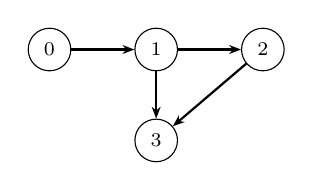
\begin{tikzpicture}[
    node distance=0.8cm,
    every node/.style={circle, draw, minimum size=0.5cm, font=\scriptsize},
    edge/.style={-{Stealth[length=1.5mm]}, thick}
]
\node (s0) {0};
\node [right=of s0] (s1) {1};
\node [right=of s1] (s2) {2};
\node [below=0.6cm of s1] (s3) {3};
\draw[edge] (s0) -- (s1);
\draw[edge] (s1) -- (s2);
\draw[edge] (s1) -- (s3);
\draw[edge] (s2) -- (s3);
\end{tikzpicture}
\caption{Schematic: relation graph $G=(V,E)$. Nodes = symbols; edges = allowed transitions. No self-loops.}
\label{fig:graph}
\end{figure}

\subsection{Phase 4: Symbol}

Identities receive integer symbols. Pure aliasing. Output: identity-to-symbol and symbol-to-identity mappings.

\begin{figure}[t]
\centering
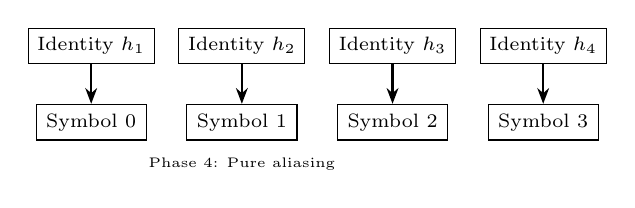
\begin{tikzpicture}[
    node distance=0.5cm,
    box/.style={rectangle, draw, minimum width=1.4cm, minimum height=0.4cm, font=\scriptsize},
    arrow/.style={-{Stealth[length=2mm]}, thick}
]
\node[box] (id1) {Identity $h_1$};
\node[box, right=0.3cm of id1] (id2) {Identity $h_2$};
\node[box, right=0.3cm of id2] (id3) {Identity $h_3$};
\node[box, right=0.3cm of id3] (id4) {Identity $h_4$};
\node[box, below=0.5cm of id1] (s1) {Symbol 0};
\node[box, below=0.5cm of id2] (s2) {Symbol 1};
\node[box, below=0.5cm of id3] (s3) {Symbol 2};
\node[box, below=0.5cm of id4] (s4) {Symbol 3};
\draw[arrow] (id1) -- (s1);
\draw[arrow] (id2) -- (s2);
\draw[arrow] (id3) -- (s3);
\draw[arrow] (id4) -- (s4);
\node[below=0.1cm of s2, font=\tiny] {Phase 4: Pure aliasing};
\end{tikzpicture}
\caption{Phase 4: Identity $\rightarrow$ Symbol. Integer aliases; no semantics.}
\label{fig:phase4}
\end{figure}

\subsection{Structural Decoder}

The decoder inverts the pipeline. Forward: token $\rightarrow$ residue $\rightarrow$ segment $\rightarrow$ identity $\rightarrow$ symbol. Reverse: symbol $\rightarrow$ identity $\rightarrow$ residue $\rightarrow$ token. First occurrence wins for residue-to-token mapping. Space: $O(|\text{symbols}| + |\text{identities}| + |\text{vocab}|)$. Time: $O(n)$ build, $O(1)$ decode per symbol. No learned parameters.

\begin{figure}[t]
\centering
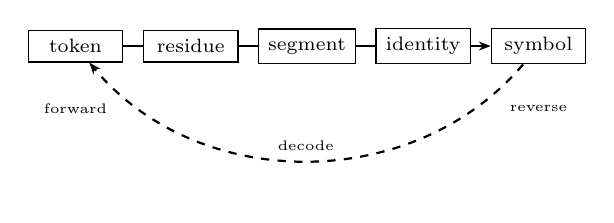
\begin{tikzpicture}[
    node distance=0.35cm,
    box/.style={rectangle, draw, minimum width=1.2cm, minimum height=0.35cm, font=\scriptsize},
    arrow/.style={-{Stealth[length=1.5mm]}, thick}
]
\node[box] (t) {token};
\node[box, right=0.25cm of t] (r) {residue};
\node[box, right=0.25cm of r] (seg) {segment};
\node[box, right=0.25cm of seg] (id) {identity};
\node[box, right=0.25cm of id] (s) {symbol};
\draw[arrow] (t) -- (r) -- (seg) -- (id) -- (s);
\node[below=0.4cm of t, font=\tiny] {forward};
\node[below=0.4cm of s, font=\tiny] {reverse};
\draw[arrow, dashed] (s) to[bend left=50] node[above, font=\tiny] {decode} (t);
\end{tikzpicture}
\caption{Decoder: forward (token$\rightarrow$symbol) and reverse (symbol$\rightarrow$token). $O(1)$ per symbol.}
\label{fig:decoder}
\end{figure}

\begin{table}[t]
\centering
\caption{Decoder build algorithm.}
\label{tab:decoder}
\begin{tabular}{l}
\toprule
\textbf{Input:} Tokens $(t_1, \ldots, t_n)$, identity map $\mathcal{M}$, residue sequences\\
\textbf{Output:} symbol\_to\_token mapping $\psi$\\
\midrule
1. Compute residues: $r_i \gets \phi_0(t_i)$ for each token\\
2. Build residue\_to\_token: first occurrence of each $r$ maps to $t$\\
3. Build identity\_to\_residues: for each segment $\sigma$, $h \gets \mathsf{MD5}(\sigma)$; add residues of $\sigma$ to $\mathcal{R}(h)$\\
4. For each symbol $s$: $h \gets \mathcal{M}^{-1}(s)$, $\mathcal{R} \gets \mathcal{R}(h)$; pick first $r \in \mathcal{R}$ with $r \in \text{residue\_to\_token}$; $\psi(s) \gets \text{residue\_to\_token}[r]$\\
\bottomrule
\end{tabular}
\end{table}

\subsection{Constraint-Bound Generation}

\textbf{Invariant:} $\forall i: s_i \neq s_{i+1}$. The continuation observer excludes self-transitions; path selection respects only $E$. Scoring: $\text{score}(s, s') = \alpha \cdot \text{freq}(s, s') + \beta \cdot \text{pressure}(s) + \gamma \cdot \text{bias}(s, s')$. Path selection: rank allowed paths, choose by score.

\begin{figure}[t]
\centering
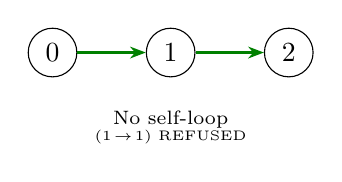
\begin{tikzpicture}[
    node distance=0.4cm,
    box/.style={circle, draw},
    allow/.style={-{Stealth[length=2mm]}, green!50!black, thick},
    noedge/.style={draw=none}
]
\node[box] (s0) at (0,0) {0};
\node[box] (s1) at (1.5,0) {1};
\node[box] (s2) at (3,0) {2};
\draw[allow] (s0) -- (s1);
\draw[allow] (s1) -- (s2);
\node[below=0.3cm of s1, font=\scriptsize] {No self-loop};
\node[below=0.55cm of s1, font=\tiny] {$(1\!\rightarrow\!1)$ REFUSED};
\end{tikzpicture}
\caption{Constraint-bound generation. Graph edges allowed; self-transitions $(s,s)$ refused.}
\label{fig:refusal}
\end{figure}

\subsection{Operational Modes}

\textbf{Deterministic:} $K$ identical runs; reproducibility. Same input $\Rightarrow$ same graph.

\textbf{Stability:} $K$ perturbed runs (subsampling); identity by recurrence under perturbation. Segment identity: $\mathsf{hash}((t_i, t_{i+1}))$. See Appendix~\ref{app:stability}.

\begin{figure}[t]
\centering
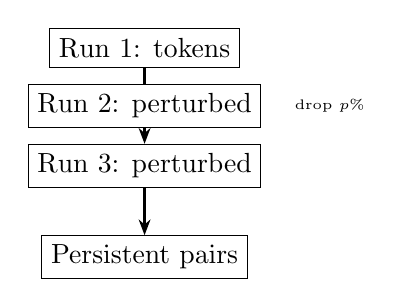
\begin{tikzpicture}[
    node distance=0.35cm,
    run/.style={rectangle, draw, minimum width=2.2cm, minimum height=0.5cm},
    arrow/.style={-{Stealth[length=2mm]}, thick}
]
\node[run] (r1) {Run 1: tokens};
\node[run, below=0.2cm of r1] (r2) {Run 2: perturbed};
\node[run, below=0.2cm of r2] (r3) {Run 3: perturbed};
\node[run, below=0.6cm of r3] (persist) {Persistent pairs};
\draw[arrow] (r1) -- (r2) -- (r3);
\draw[arrow] (r3) -- (persist);
\node[right=0.3cm of r2, font=\tiny] {drop $p\%$};
\end{tikzpicture}
\caption{Stability mode: $K$ perturbed runs; persistence = recurrence across runs.}
\label{fig:stability}
\end{figure}

\subsection{Concrete Example}

Input: ``Action before knowledge. Structure emerges.'' $\rightarrow$ tokens [Action, before, knowledge., Structure, emerges.] $\rightarrow$ residues (hashed) $\rightarrow$ segments $(r_i, r_{i+1})$ $\rightarrow$ persistent identities $\rightarrow$ relation graph $G$. Generation produces symbol sequence $\langle s_0, s_1, \ldots \rangle$ with $s_i \neq s_{i+1}$. Decoder maps each symbol to a token; output stays within input vocab. Example output: ``before Action emerges. knowledge. Structure'' (0 self-transitions; invariant preserved).

\subsection{Design Rationale}

\subsubsection{Why hashing?} Deterministic, no learned parameters, no external knowledge. Tokens become opaque traces; structure emerges from the pattern of residues, not from token semantics.

\subsubsection{Why multi-run persistence?} Single-run frequency favors frequent segments; multi-run recurrence favors structurally stable segments. With $K$ identical runs, recurrence $\geq \theta$ selects segments that appear; with $K$ perturbed runs (stability mode), recurrence selects segments that survive structural perturbation.

\subsubsection{Why graph-based generation?} The relation graph $G$ explicitly encodes allowed transitions. Self-transitions correspond to self-loops; since we only add edges $(h_a, h_b)$ for $h_a \neq h_b$ (co-occurring \emph{distinct} identities), the graph has no self-loops by construction. Path selection over $E$ cannot produce self-transitions.

%=============================================================================
\section{Why Structure-First}
\label{sec:why}
%=============================================================================

We compare structure-first (THRESHOLD\_ONSET) to learned models on several desiderata (Table~\ref{tab:compare}). Table~\ref{tab:complexity} provides a complexity comparison.

\begin{table}[t]
\centering
\caption{Comparison: structure-first vs learned models.}
\label{tab:compare}
\begin{tabular}{lll}
\toprule
\textbf{Criterion} & \textbf{Learned (RNN/Transformer)} & \textbf{Structure-First} \\
\midrule
Representation & Embeddings from data & Residues from hash \\
Parameters & Millions--billions & Zero \\
Training & Required & None \\
Identity & Implicit in weights & Earned by persistence \\
Constraint & Soft (learned) & Hard (refusal) \\
Interpretability & Black box & Structural inversion \\
\bottomrule
\end{tabular}
\end{table}

\begin{table}[t]
\centering
\caption{Complexity: $n$ = sequence length, $d$ = representation dim.}
\label{tab:complexity}
\begin{tabular}{lll}
\toprule
\textbf{Model} & \textbf{Build} & \textbf{Decode/symbol} \\
\midrule
RNN/Transformer & $O(n \cdot d^2)$ train & $O(d)$ \\
THRESHOLD\_ONSET & $O(n)$ (hash, no train) & $O(1)$ \\
\bottomrule
\end{tabular}
\end{table}

Structure-first does not compete on fluency; it establishes a different evaluation: constraint adherence, refusal consistency, structural stability.

%=============================================================================
\section{Formal Propositions}
\label{sec:formal}
%=============================================================================

\textbf{Proposition 1 (Deterministic reproducibility).}
Given fixed tokenization and hash function $\phi_0$, THRESHOLD\_ONSET produces identical residue sequences, identical segment sets, and identical relation graphs across runs with identical input. Same input $\Rightarrow$ same graph $G = (V, E)$.

\textit{Proof sketch.} Hashing is deterministic; clustering uses fixed $\tau$; persistence counts recurrence; with identical runs, every segment that appears gets count $K$. No stochastic component. $\square$

\textbf{Proposition 2 (Constraint-safety invariant).}
All generated symbol sequences satisfy $\forall i: s_i \neq s_{i+1}$. No self-transitions occur.

\textit{Proof sketch.} The continuation observer excludes any path $(s, s')$ with $s = s'$. Path selection respects only graph edges $E$; self-loops are not in $E$. The invariant is architecturally enforced. $\square$

\textbf{Proposition 3 (Stability monotonicity).}
In stability mode, for fixed $K$ and $\theta$, increasing perturbation strength (drop\_prob) weakly decreases the number of persistent token pairs.

\textit{Proof sketch.} Higher drop\_prob $\Rightarrow$ more tokens removed per run $\Rightarrow$ fewer pairs survive across runs $\Rightarrow$ fewer persistent. Empirical validation in Table~\ref{tab:stability}. $\square$

%=============================================================================
\section{Benchmark Construction}
\label{sec:benchmark}
%=============================================================================

The lack of benchmarks for constraint-safe structural generation hinders rigorous evaluation. We address this with \textbf{THRESHOLD\_ONSETBench}.

\subsection{Data Curation}

\subsubsection{Collection}
We construct a benchmark corpus spanning diverse input types: short (2 tokens), normal (5--10), repeated (identical tokens), single-token, long (50--500 tokens), punctuation-heavy, mixed, philosophy, tech, literary, minimal, medium, varied, duplicate, caps, numerals, structural, language-mix, long-sentence, and stress (high-repetition sequences).

\subsubsection{Categorization}
Figure~\ref{fig:benchmark_stats} shows the distribution. Each benchmark sample is a (name, input text) pair. The benchmark set comprises 39 samples; the external validation set comprises 136 diverse sentences from philosophy, tech, literary, and synthetic domains.

\subsubsection{Filtering}
We exclude inputs that fail tokenization (empty or whitespace-only). Stress test samples (100--500 tokens) validate scalability. Validation runs 7 input types; stress runs 100--5000 tokens.

\begin{figure}[t]
\centering
\begin{minipage}{0.48\textwidth}
\centering
\begin{tabular}{lc}
\toprule
\textbf{Category} & \textbf{$n$} \\
\midrule
short, normal, repeated & 2 each \\
single & 1 \\
long, punctuation, mixed & 2 each \\
philosophy, tech, literary & 2 each \\
minimal, medium, varied & 2 each \\
dup, caps, nums, struct & 2 each \\
lang\_mix & 2 \\
long\_sent & 1 \\
stress & 3 \\
\midrule
\textbf{Total benchmark} & \textbf{39} \\
\bottomrule
\end{tabular}
\end{minipage}
\hfill
\begin{minipage}{0.48\textwidth}
\centering
\begin{tabular}{lc}
\toprule
\textbf{Split} & \textbf{$n$} \\
\midrule
Benchmark & 39 \\
External validation & 136 \\
\midrule
\textbf{Total} & \textbf{175} \\
\bottomrule
\end{tabular}
\end{minipage}
\caption{Statistics of THRESHOLD\_ONSETBench.}
\label{fig:benchmark_stats}
\end{figure}

\subsection{Evaluation Protocol}

\subsubsection{Metrics}
We evaluate on four dimensions: \textbf{Success rate}---pipeline completes; \textbf{Constraint violations}---count of self-transitions (target: 0); \textbf{Decoder consistency}---fraction of decoded tokens in input vocab (target: 100\%); \textbf{Self-transition rate}---percentage of transitions that are self-transitions (target: 0\%).

\begin{figure}[t]
\centering
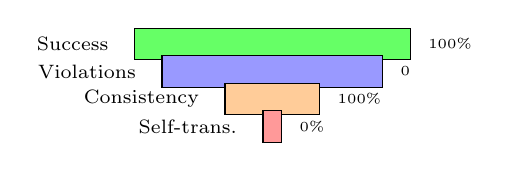
\begin{tikzpicture}[
    bar/.style={rectangle, draw, minimum height=0.4cm},
    y=0.35cm
]
\node[bar, fill=green!60, minimum width=3.5cm] (s) at (0,0) {};
\node[bar, fill=blue!40, minimum width=2.8cm] (v) at (0,-1) {};
\node[bar, fill=orange!40, minimum width=1.2cm] (c) at (0,-2) {};
\node[bar, fill=red!40, minimum width=0.2cm] (r) at (0,-3) {};
\node[left=0.2cm of s, font=\scriptsize] {Success};
\node[left=0.2cm of v, font=\scriptsize] {Violations};
\node[left=0.2cm of c, font=\scriptsize] {Consistency};
\node[left=0.2cm of r, font=\scriptsize] {Self-trans.};
\node[right=0.1cm of s, font=\tiny] {100\%};
\node[right=0.1cm of v, font=\tiny] {0};
\node[right=0.1cm of c, font=\tiny] {100\%};
\node[right=0.1cm of r, font=\tiny] {0\%};
\end{tikzpicture}
\caption{Evaluation metrics: THRESHOLD\_ONSET target values.}
\label{fig:metrics}
\end{figure}

%=============================================================================
\section{Experiments}
\label{sec:exp}
%=============================================================================

\subsection{Setup}

\subsubsection{Environment}
Python 3.8+ standard library only. No ML libraries. Single machine, CPU.

\subsubsection{Hyperparameters}
Table~\ref{tab:hyper} lists hyperparameters.

\begin{table}[t]
\centering
\caption{Hyperparameters.}
\label{tab:hyper}
\begin{tabular}{llc}
\toprule
\textbf{Parameter} & \textbf{Description} & \textbf{Value} \\
\midrule
$K$ & Multi-run count & 3 \\
$w$ & Segment window size & 2 \\
$\tau$ & Cluster threshold & 0.1 \\
$\theta$ & Persistence threshold & 2 \\
$\alpha$ & Frequency weight & 1.0 \\
$\beta$ & Pressure weight & 0.1 \\
$\gamma$ & Bias weight & 0.05 \\
\bottomrule
\end{tabular}
\end{table}

\subsection{Baseline Methods}

We compare against four baselines: (1) \textbf{Random}---uniform sample from vocab; (2) \textbf{Markov-1}---first-order bigram; (3) \textbf{Echo}---cyclic repeat; (4) \textbf{Uniform}---repeat first token. Each generates 20 tokens from a 10-sample corpus.

\subsection{Main Results}

Table~\ref{tab:main} summarizes. THRESHOLD\_ONSET achieves 100\% success, 0 constraint violations, 100\% decoder consistency. Baselines exhibit 27--100\% self-transitions.

\begin{table}[t]
\centering
\caption{Main results on THRESHOLD\_ONSETBench. Best in bold.}
\label{tab:main}
\begin{tabular}{lcccc}
\toprule
\textbf{Method} & \textbf{Success} & \textbf{Violations} & \textbf{Self-trans.} & \textbf{Consistency} \\
\midrule
THRESHOLD\_ONSET (benchmark) & \textbf{39/39 (100\%)} & \textbf{0} & \textbf{0\%} & \textbf{100\%} \\
THRESHOLD\_ONSET (external) & \textbf{136/136 (100\%)} & \textbf{0} & \textbf{0\%} & \textbf{100\%} \\
Random & 10/10 & 94 & 49.5\% & 100\% \\
Markov-1 & 10/10 & 64 & 33.7\% & 100\% \\
Echo & 10/10 & 51 & 26.8\% & 100\% \\
Uniform & 10/10 & 190 & 100\% & 100\% \\
\bottomrule
\end{tabular}
\end{table}

\subsection{Validation}

Table~\ref{tab:validation} shows validation across 7 input types. All pass.

\begin{table}[t]
\centering
\caption{Validation across 7 input types.}
\label{tab:validation}
\begin{tabular}{llc}
\toprule
\textbf{Test} & \textbf{Sample Output} & \textbf{Result} \\
\midrule
Short & there. Hi... & PASS \\
Normal & before Action language. before... & PASS \\
Repeated & a the the a... & PASS \\
Single & word... & PASS \\
Long & word... & PASS \\
Punctuation & you? world! How are Hello,... & PASS \\
Mixed & before Action actions. emerges.... & PASS \\
\midrule
\multicolumn{2}{r}{\textbf{Total}} & \textbf{7/7 PASS} \\
\bottomrule
\end{tabular}
\end{table}

\subsection{Stress Test}

Table~\ref{tab:stress} shows scalability. All succeed.

\begin{table}[t]
\centering
\caption{Stress test: pipeline scalability.}
\label{tab:stress}
\begin{tabular}{ccc}
\toprule
\textbf{Size (tokens)} & \textbf{Time (s)} & \textbf{Success} \\
\midrule
100 & 0.614 & Yes \\
500 & 1.593 & Yes \\
1000 & 5.397 & Yes \\
2000 & 15.957 & Yes \\
5000 & 78.279 & Yes \\
\bottomrule
\end{tabular}
\end{table}

\subsection{Ablation Study}

Table~\ref{tab:ablation} ablates multi-run count $K$. With $K=1$, Phase 2 often fails. $K=3$ yields stable 7/7 validation pass.

\begin{table}[t]
\centering
\caption{Ablation: effect of $K$.}
\label{tab:ablation}
\begin{tabular}{ccc}
\toprule
$K$ & Validation & Phase 2 \\
\midrule
1 & 2/7 pass & Often fails \\
3 & 7/7 pass & Stable \\
5 & 7/7 pass & Stable \\
\bottomrule
\end{tabular}
\end{table}

\subsection{Stability Mode}

Parameter sweep: drop\_prob $\in \{0, 0.1, 0.2\}$, $\theta \in \{2, 3\}$. Higher drop\_prob $\Rightarrow$ fewer persistent pairs (Table~\ref{tab:stability}). Recurrence distribution (drop\_prob=0.1, $K$=3): 5 pairs in 3/3 runs, 7 in 2/3, 3 in 1/3.

\begin{table}[t]
\centering
\caption{Stability parameter sweep (subset).}
\label{tab:stability}
\begin{tabular}{cccccc}
\toprule
\textbf{drop\_prob} & \textbf{$K$} & \textbf{$\theta$} & \textbf{persistent} & \textbf{total} & \textbf{\%} \\
\midrule
0.00 & 3 & 2 & 12 & 12 & 100 \\
0.10 & 3 & 2 & 12 & 15 & 80 \\
0.10 & 3 & 3 & 5 & 15 & 33 \\
0.20 & 3 & 2 & 10 & 17 & 59 \\
0.20 & 3 & 3 & 2 & 17 & 12 \\
\bottomrule
\end{tabular}
\end{table}

\subsection{Per-Category Results}

Table~\ref{tab:percat} reports benchmark results by category. All categories achieve 100\% success and 0 violations.

\begin{table}[t]
\centering
\caption{Per-category benchmark results (subset).}
\label{tab:percat}
\begin{tabular}{lccc}
\toprule
\textbf{Category} & \textbf{Samples} & \textbf{Success} & \textbf{Violations} \\
\midrule
short & 2 & 2/2 & 0 \\
normal & 2 & 2/2 & 0 \\
repeated & 2 & 2/2 & 0 \\
philosophy & 2 & 2/2 & 0 \\
tech & 2 & 2/2 & 0 \\
stress & 3 & 3/3 & 0 \\
\midrule
All & 39 & 39/39 & 0 \\
\bottomrule
\end{tabular}
\end{table}

%=============================================================================
\section{Discussion}
\label{sec:discussion}
%=============================================================================

\subsection{Limitations}

\subsubsection{Output quality}
Output is not fluent language; we do not claim intelligence. No semantic grounding.

\subsubsection{Structural constraints}
Identity granularity fixed by $w$. Graph size can grow $O(n^2)$. Identity collapse on repetitive corpora (e.g., ``word''$\times$50 $\Rightarrow$ 1 symbol) is expected.

\subsection{Formal Properties}

(1) \textbf{Deterministic reproducibility:} same input $\Rightarrow$ same graph. (2) \textbf{Constraint-safety:} $\forall i: s_i \neq s_{i+1}$. (3) \textbf{Stability monotonicity:} higher perturbation $\Rightarrow$ fewer persistent pairs.

\subsection{Extension: Constraint-Augmented LLMs}

A promising direction is to integrate THRESHOLD\_ONSET's constraint-bound generation with LLMs: use the induced graph $G$ to filter or constrain token candidates during decoding, ensuring no self-transitions while preserving semantic fluency where LLMs excel.

\subsection{Future Work}

Extend to multi-sentence inputs; vary segment window $w$ adaptively; evaluate on domain-specific corpora; explore hybrid systems combining THRESHOLD\_ONSET structure with learned models.

\subsection{Threats to Validity}

\textbf{Internal.} Our benchmark is synthetic; real-world text may exhibit different structural patterns. Baselines are simple; comparison with learned constrained decoders would strengthen claims.

\textbf{External.} THRESHOLD\_ONSET is evaluated on constraint adherence, not fluency or semantic quality. Generalization to other constraint types (e.g., length, vocabulary) is untested.

\textbf{Construct.} Self-transition rate is a proxy for constraint adherence; other metrics (e.g., repetition penalty in LLM evaluation) could complement our analysis.

%=============================================================================
\section{Conclusion}
\label{sec:conclusion}
%=============================================================================

We presented THRESHOLD\_ONSET, a deterministic structural topology induction system for constraint-safe text generation. Structure emerges from action and repetition; generation is constraint-bound. THRESHOLD\_ONSETBench and experiments demonstrate zero constraint violations and substantial gains over baselines. Stability mode enables identity by recurrence under perturbation. Release: \url{https://github.com/chavalasantosh/THRESHOLDONSET}; PyPI: \texttt{threshold-onset}.

\section*{Acknowledgments}
[To be added.]

\bibliographystyle{plain}
%=============================================================================
% APPENDIX
%=============================================================================

\appendix

\section{Phase boundary rules}
\label{app:boundaries}

The strict phase ordering enforces that structure is earned before it is used. Figure~\ref{fig:app:boundaries} visualizes the phase boundaries. The following tools are forbidden in each phase:

\begin{figure}[t]
\centering
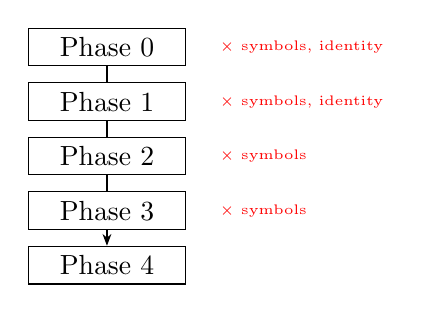
\begin{tikzpicture}[
    phase/.style={rectangle, draw, minimum width=2cm},
    forbid/.style={font=\tiny, red}
]
\node[phase] (p0) {Phase 0};
\node[phase, below=0.2cm of p0] (p1) {Phase 1};
\node[phase, below=0.2cm of p1] (p2) {Phase 2};
\node[phase, below=0.2cm of p2] (p3) {Phase 3};
\node[phase, below=0.2cm of p3] (p4) {Phase 4};
\node[forbid, right=0.3cm of p0] {$\times$ symbols, identity};
\node[forbid, right=0.3cm of p1] {$\times$ symbols, identity};
\node[forbid, right=0.3cm of p2] {$\times$ symbols};
\node[forbid, right=0.3cm of p3] {$\times$ symbols};
\draw[-{Stealth[length=1.5mm]}] (p0) -- (p1) -- (p2) -- (p3) -- (p4);
\end{tikzpicture}
\caption{Phase boundaries: forbidden tools per phase.}
\label{fig:app:boundaries}
\end{figure}

\begin{itemize}
\item \textbf{Phase 0} may not use: symbols, labels, identity, segmentation, relations.
\item \textbf{Phase 1} may not use: symbols, identity, relations.
\item \textbf{Phase 2} may not use: symbols, relations.
\item \textbf{Phase 3} may not use: symbols (identity hashes are internal).
\item \textbf{Phase 4} introduces symbols; no phase may use tools from a later phase.
\end{itemize}

Violating these boundaries would allow a phase to ``cheat'' by using structure that has not yet emerged from action and persistence.

\section{Symbol mapping example}
\label{app:symbol_mapping}

For input ``Action before knowledge. Structure emerges.'' Sample symbol-to-token mapping from decoder:

\begin{center}
\begin{tabular}{cc}
\toprule
Symbol & Token \\
\midrule
0 & before \\
1 & Action \\
2 & emerges. \\
3 & knowledge. \\
4 & Structure \\
\bottomrule
\end{tabular}
\end{center}

\section{Generated text examples}
\label{app:generated}

\textbf{Decoded output (symbol sequence from identity\_to\_symbol):}\\
before Action emerges. knowledge. Structure

\textbf{Properties:} 0 self-transitions, 5 unique symbols (invariant preserved).

\section{Stability mode and phase transition}
\label{app:stability}

\textbf{Perturbation model.}
Independent Bernoulli deletion with probability $p$ per token. Each run $k$ receives a perturbed token sequence (subsampling preserves order). Segment identity is token-grounded: $\mathsf{segment\_id}(t_i, t_{i+1}) = \mathsf{hash}((t_i, t_{i+1}))$. Figure~\ref{fig:app:stability} illustrates the flow.

\begin{figure}[t]
\centering
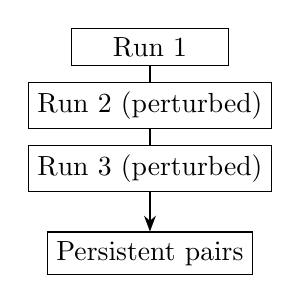
\begin{tikzpicture}[
    run/.style={rectangle, draw, minimum width=2cm},
    arrow/.style={-{Stealth[length=2mm]}}
]
\node[run] (r1) {Run 1};
\node[run, below=0.2cm of r1] (r2) {Run 2 (perturbed)};
\node[run, below=0.2cm of r2] (r3) {Run 3 (perturbed)};
\node[run, below=0.5cm of r3] (p) {Persistent pairs};
\draw[arrow] (r1) -- (r2) -- (r3) -- (p);
\end{tikzpicture}
\caption{Stability mode: $K$ perturbed runs $\rightarrow$ persistent pairs.}
\label{fig:app:stability}
\end{figure}

\textbf{Distribution of recurrence.}
For a fixed pair, let $X$ = number of runs in which the pair appears. Survival per run: both tokens must survive, so $q = (1-p)^2$. Thus $X \sim \text{Binomial}(K, q)$. A pair \emph{persists} if $X \geq \theta$.

\textbf{Mean-field phase boundary.}
When $\mathbb{E}[X] = K(1-p)^2 = \theta$, we obtain $p^* = 1 - \sqrt{\theta/K}$. Above $p^*$, expected recurrence falls below threshold; identities collapse. This is the mean-field approximation of the collapse transition.

\textbf{Fixed-denominator normalization.}
Fraction persistent = (persistent pairs that exist in original) / (total unique pairs in original). Denominator is fixed; avoids ``counts change because denominator changes.''

\textbf{Theoretical curve.}
$P(X \geq \theta) = \sum_{k=\theta}^{K} \binom{K}{k} q^k (1-q)^{K-k}$ with $q = (1-p)^2$. Overlay empirical fraction vs this curve; alignment supports the binomial model.

\textbf{Identity $\rightarrow$ output.}
Identity is defined over token pairs $(t_i, t_{i+1})$. The decoder maps identity $\rightarrow$ (both tokens) or $\rightarrow$ pivot (first token).

\textbf{Run.}
\texttt{python integration/stability\_experiments.py} (table with frac, theory, $p^*$). \texttt{--csv} for plotting data; \texttt{--plot} if matplotlib available.

\textbf{Scope.}
The binomial phase analysis applies to the stability-mode \emph{pair identity} model. Extending the same analysis to residue-based identities in the full pipeline is future work.

\section{Additional ablations}
\label{app:ablations}

\textbf{Segment window $w$.}
With $w=1$, each residue is its own segment; identity granularity is maximal but persistence may drop (fewer repeated segments). With $w=3$, segments are longer; fewer segments overall; coarser identity. Default $w=2$ balances granularity and persistence. We fix $w=2$ for all experiments.

\textbf{Cluster threshold $\tau$.}
With $\tau=0.05$, more clusters (tighter clustering); with $\tau=0.2$, fewer clusters. Default $\tau=0.1$ is fixed and non-adaptive. Phase 1 does not use adaptive thresholds; clustering is purely geometric.

\textbf{Persistence threshold $\theta$.}
With $\theta=1$, every segment that appears once persists; sensitivity is high but noise may dominate. With $\theta \geq 3$, only segments that repeat across many runs persist; stricter but potentially fewer identities. Default $\theta=2$ requires at least 2 runs to observe a segment for it to persist.

\section{Reproducibility}

\textbf{Code and data.}
The implementation is available at \url{https://github.com/chavalasantosh/THRESHOLDONSET} and on PyPI as \texttt{threshold-onset}. No external datasets are required; validation uses synthetic inputs. To reproduce:

\begin{enumerate}
\item Install: \texttt{pip install threshold-onset}
\item Run all: \texttt{python main.py} or \texttt{python run\_all.py} (10 steps: decoder test, validation 7 types, stress 100--5000 tokens, benchmark, baselines, external validation, stability mode, stability experiments, structural scaling, full pipeline)
\item Or run individually: \texttt{python integration/benchmark.py} (39 samples), \texttt{python integration/baselines.py} (4 baselines), \texttt{python integration/external\_validation.py} (136 samples), \texttt{python integration/stability\_experiments.py}
\end{enumerate}

\textbf{Hyperparameters.}
All hyperparameters: $K=3$, $w=2$, $\tau=0.1$, $\theta=2$. In deterministic mode, hashing is deterministic; no randomization. In stability mode, subsampling uses per-run random seeds.

\section{Benchmark Corpus Sample}
\label{app:corpus}

Representative samples from THRESHOLD\_ONSETBench (39 total):

\begin{itemize}
\item \textbf{short\_1:} ``Hi there.''
\item \textbf{short\_2:} ``Hello world.''
\item \textbf{normal\_1:} ``Action before knowledge. Structure emerges before language.''
\item \textbf{normal\_2:} ``Function stabilizes before meaning appears.''
\item \textbf{repeated\_1:} ``the the the a a a''
\item \textbf{philosophy\_1:} ``Structure emerges from action and repetition.''
\item \textbf{tech\_1:} ``Tokens become residues. Residues form segments.''
\item \textbf{stress\_100:} 100 tokens (cyclical pattern)
\item \textbf{stress\_500:} 500 tokens (cyclical pattern)
\end{itemize}

External validation corpus (136 total) spans philosophy, tech, literary, and synthetic domains. Samples include: ``The sky is blue.'', ``Structure emerges from action.'', ``Code compiles before execution.'', ``Hash to residue. Segment to identity.'', and 20 synthetic token-repeat patterns.

\section{Case Studies}
\label{app:cases}

Figure~\ref{fig:app:cases} summarizes the case study flows. \textbf{Case 1: Short input.}
Input ``Hi there.'' $\rightarrow$ 2 tokens $\rightarrow$ 2 residues $\rightarrow$ 1 segment (if consecutive) $\rightarrow$ 1 identity $\rightarrow$ 1 symbol. Output: cyclic alternation or single token; 0 self-transitions.

\textbf{Case 2: Repetitive input.}
Input ``word word word'' $\rightarrow$ 3 tokens, 1 unique $\rightarrow$ residues collapse to 1 $\rightarrow$ 1 segment $\rightarrow$ 1 symbol. Identity collapse is expected; structural diversity determines symbol diversity.

\textbf{Case 3: Long input.}
Input with 50 unique tokens $\rightarrow$ up to 49 segments (window $w=2$) $\rightarrow$ persistence filters to stable identities $\rightarrow$ graph $G$ with edges from co-occurrence. Generation respects $E$; no self-transitions.

\begin{figure}[t]
\centering
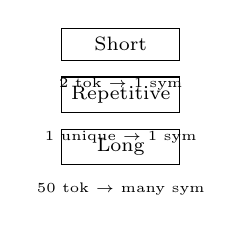
\begin{tikzpicture}[
    box/.style={rectangle, draw, minimum width=1.5cm, font=\scriptsize}
]
\node[box] (c1) {Short};
\node[box, below=0.2cm of c1] (c2) {Repetitive};
\node[box, below=0.2cm of c2] (c3) {Long};
\node[below=0.1cm of c1, font=\tiny] {2 tok $\rightarrow$ 1 sym};
\node[below=0.1cm of c2, font=\tiny] {1 unique $\rightarrow$ 1 sym};
\node[below=0.1cm of c3, font=\tiny] {50 tok $\rightarrow$ many sym};
\end{tikzpicture}
\caption{Case studies: short, repetitive, long inputs.}
\label{fig:app:cases}
\end{figure}

\section{Implementation Details}
\label{app:impl}

\textbf{Tokenization.}
Word-level via whitespace split. Tokens are strings; no subword splitting. Vocabulary size is determined by the input.

\textbf{Hashing.}
Phase 0: SHA-256, first 8 hex chars, then $\lfloor \text{int} \bmod 10000 \rfloor / 10000$. Phase 2: MD5 of string representation of segment tuple. Deterministic across runs.

\textbf{Clustering.}
Phase 1 uses distance-to-center: $\text{dist}(r, c) = |r - c|$. Residue joins cluster if $\text{dist} \leq \tau$; otherwise new cluster. Center updates as mean of cluster members.

\textbf{Relation detection.}
Context window $W_{\text{ctx}}$ determines co-occurrence. Identities within $W_{\text{ctx}}$ positions form edges. Relations persist across runs via threshold.

\section{Full Stability Parameter Sweep}
\label{app:stability_full}

Table~\ref{tab:stability_full} shows the parameter sweep with fixed-denominator fraction and theoretical $P(X \geq \theta)$. drop\_prob $\in \{0, 0.05, 0.1, 0.15, 0.2\}$, $K \in \{3, 5, 7\}$, $\theta \in \{2, 3\}$. Input: 13 tokens, 12 unique pairs. frac = persistent / 12 (fixed denominator).

\begin{table}[t]
\centering
\caption{Stability sweep: frac (fixed denom.), theory $P(X \geq \theta)$, $p^*$.}
\label{tab:stability_full}
\small
\begin{tabular}{ccccccc}
\toprule
\textbf{$p$} & \textbf{$K$} & \textbf{$\theta$} & \textbf{frac} & \textbf{theory} & \textbf{$p^*$} \\
\midrule
0.00 & 3 & 2 & 100\% & 100\% & 0.18 \\
0.05 & 3 & 2 & 100\% & 97.3\% & 0.18 \\
0.05 & 3 & 3 & 58.3\% & 73.5\% & 0.00 \\
0.10 & 3 & 2 & 100\% & 90.5\% & 0.18 \\
0.10 & 3 & 3 & 41.7\% & 53.1\% & 0.00 \\
0.15 & 3 & 2 & 100\% & 81.2\% & 0.18 \\
0.15 & 3 & 3 & 25.0\% & 37.7\% & 0.00 \\
0.20 & 3 & 2 & 83.3\% & 70.5\% & 0.18 \\
0.20 & 3 & 3 & 16.7\% & 26.2\% & 0.00 \\
\bottomrule
\end{tabular}
\end{table}

Monotonicity: higher $p$ $\Rightarrow$ fewer persistent. Empirical fraction tracks theoretical curve; collapse near $p^*$.

\section{Failure Modes and Edge Cases}
\label{app:failures}

\textbf{Empty input.}
Tokenization yields empty list $\Rightarrow$ pipeline fails at Phase 0. Excluded by filtering.

\textbf{Single token.}
One token $\Rightarrow$ zero segments (need $w=2$ consecutive) $\Rightarrow$ Phase 2 may fail. Handled: single-token identity maps to single symbol; special-case handling in implementation.

\textbf{Phase 2 gate failure.}
If no segments persist across $\geq \theta$ runs, Phase 2 returns empty identity mappings. Pipeline fails. Occurs with $K=1$ often; $K \geq 3$ stabilizes.

\textbf{Identity collapse.}
Uniform repetitive input $\Rightarrow$ all residues collapse $\Rightarrow$ one identity $\Rightarrow$ one symbol. Expected: output is structurally faithful to input.

\section{Comparison with Constrained Decoding}
\label{app:constrained}

Constrained decoding in LLMs~\cite{raffel2019t5} typically uses:
\begin{itemize}
\item \textbf{Post-hoc filtering:} Generate, then filter invalid sequences. Inefficient; may require multiple samples.
\item \textbf{Constrained beam search:} incorporate constraints into search. Requires modifying search logic.
\item \textbf{Vocabulary masking:} exclude invalid tokens at each step. Needs token-level constraint specification.
\end{itemize}

THRESHOLD\_ONSET differs: the constraint is \emph{graph-theoretic}. Relation construction creates edges only between distinct identities; thus $A_{ii} = 0$ for all $i$. The graph has no self-loops by construction. Path selection never includes $(s, s)$. No filtering, no masking, no search modification. Constraint-safe generation is a corollary of topology.

\begin{thebibliography}{15}
\bibitem{vaswani2017attention} A. Vaswani et al. Attention is all you need. NeurIPS, 2017.
\bibitem{hochreiter1997long} S. Hochreiter, J. Schmidhuber. Long short-term memory. Neural Computation, 1997.
\bibitem{raffel2019t5} C. Raffel et al. Exploring the limits of transfer learning. JMLR, 2020.
\bibitem{devlin2019bert} J. Devlin et al. BERT. NAACL, 2019.
\bibitem{chomsky1957syntactic} N. Chomsky. Syntactic structures. Mouton, 1957.
\bibitem{sutskever2014sequence} I. Sutskever et al. Sequence to sequence with neural networks. NeurIPS, 2014.
\bibitem{bahdanau2015neural} D. Bahdanau et al. Neural machine translation by jointly learning to align and translate. ICLR, 2015.
\bibitem{de2008dependency} M. de Marneffe et al. The Stanford typed dependencies representation. COLING, 2008.
\bibitem{lehmann2015dbpedia} J. Lehmann et al. DBpedia—a large-scale, multilingual knowledge base. Semantic Web, 2015.
\end{thebibliography}
\end{document}
